\documentclass[landscape,final,a0paper,fontscale=0.285]{baposter}

\usepackage{calc}
\usepackage{graphicx} % Required for including images
\usepackage{amsmath}  % For typesetting math
\usepackage{amssymb}  % Adds new symbols to be used in math mode
\usepackage{relsize}  % Chagnge size of text /smaller, /larger
\usepackage{multirow} % Allows table cells to span more than one row of the table
\usepackage{rotating} % Rotate figures and tables
\usepackage{bm}       % Allows a math expression to be bold
\usepackage{url}      % Allows email address and websites

\usepackage{float}
\usepackage{caption} % Required for specifying captions to tables and figures
\usepackage{wrapfig} % Wrap text around figure
\usepackage[export]{adjustbox}

\captionsetup[figure]{font=Large,skip=0pt,labelformat=empty,justification=raggedright,singlelinecheck=false}

\usepackage{multicol} % Required for multiple columns

\usepackage[utf8]{inputenc} %Required for IEEE reference style
\newcommand{\BIBdecl}{\setlength{\itemsep}{-0.25 em}} %Removes line space between references

%\usepackage{times}
%\usepackage{helvet}
%\usepackage{bookman}
\usepackage{palatino}

%\newcommand{\captionfont}{\footnotesize}

\graphicspath{{images/}{../images/}}
%\usetikzlibrary{calc}

\newcommand{\SET}[1]  {\ensuremath{\mathcal{#1}}}
\newcommand{\MAT}[1]  {\ensuremath{\boldsymbol{#1}}}
\newcommand{\VEC}[1]  {\ensuremath{\boldsymbol{#1}}}
\newcommand{\Video}{\SET{V}}
\newcommand{\video}{\VEC{f}}
\newcommand{\track}{x}
\newcommand{\Track}{\SET T}
\newcommand{\LMs}{\SET L}
\newcommand{\lm}{l}
\newcommand{\PosE}{\SET P}
\newcommand{\posE}{\VEC p}
\newcommand{\negE}{\VEC n}
\newcommand{\NegE}{\SET N}
\newcommand{\Occluded}{\SET O}
\newcommand{\occluded}{o}

%%%%%%%%%%%%%%%%%%%%%%%%%%%%%%%%%%%%%%%%%%%%%%%%%%%%%%%%%%%%%%%%%%%%%%%%%%%%%%%%
% Multicol Settings
%%%%%%%%%%%%%%%%%%%%%%%%%%%%%%%%%%%%%%%%%%%%%%%%%%%%%%%%%%%%%%%%%%%%%%%%%%%%%%%%
\setlength{\columnsep}{1.5em}
\setlength{\columnseprule}{0mm}

%%%%%%%%%%%%%%%%%%%%%%%%%%%%%%%%%%%%%%%%%%%%%%%%%%%%%%%%%%%%%%%%%%%%%%%%%%%%%%%%
% Save space in lists. Use this after the opening of the list
%%%%%%%%%%%%%%%%%%%%%%%%%%%%%%%%%%%%%%%%%%%%%%%%%%%%%%%%%%%%%%%%%%%%%%%%%%%%%%%%
\newcommand{\compresslist}{%
\setlength{\itemsep}{1pt}%
\setlength{\parskip}{0pt}%
\setlength{\parsep}{0pt}%
}

%%%%%%%%%%%%%%%%%%%%%%%%%%%%%%%%%%%%%%%%%%%%%%%%%%%%%%%%%%%%%%%%%%%%%%%%%%%%%%
%%% Begin of Document
%%%%%%%%%%%%%%%%%%%%%%%%%%%%%%%%%%%%%%%%%%%%%%%%%%%%%%%%%%%%%%%%%%%%%%%%%%%%%%

\begin{document}

%%%%%%%%%%%%%%%%%%%%%%%%%%%%%%%%%%%%%%%%%%%%%%%%%%%%%%%%%%%%%%%%%%%%%%%%%%%%%%
%%% Here starts the poster
%%%---------------------------------------------------------------------------
%%% Format it to your taste with the options
%%%%%%%%%%%%%%%%%%%%%%%%%%%%%%%%%%%%%%%%%%%%%%%%%%%%%%%%%%%%%%%%%%%%%%%%%%%%%%
% Define some colors

%\definecolor{lightblue}{cmyk}{0.83,0.24,0,0.12}
\definecolor{lightblue}{rgb}{0.145,0.6666,1}

%%
\begin{poster}%
  % Poster Options
  {
  % Show grid to help with alignment
  grid=false,
  % Column spacing
  colspacing=1em,
  % Color style
  bgColorOne=white,
  bgColorTwo=white,
  borderColor=lightblue,
  headerColorOne=black,
  headerColorTwo=lightblue,
  headerFontColor=white,
  boxColorOne=white,
  boxColorTwo=lightblue,
  % Format of textbox
  textborder=roundedleft,
  % Format of text header
  eyecatcher=true,
  headerborder=closed,
  headerheight=0.1\textheight,
%  textfont=\sc, An example of changing the text font
  headershape=roundedright,
  headershade=shadelr,
  headerfont=\Large\bf\textsc, %Sans Serif
  textfont={\setlength{\parindent}{1.5em}},
  boxshade=plain,
%  background=shade-tb,
  background=plain,
  linewidth=2pt
  }

    % University logo
 % {
\includegraphics[height=4em]{img/penn_state_cla_logo_new_210-89.jpg}}
  % Title
  {\bf{School-age children perceive fast radial optic flow in noise more accurately than slow linear flow} \vspace{0.2em}}
  % Authors
  {Rick O. Gilmore \emph{(rogilmore@psu.edu)}, Michelle A. Shade, Michael J. O'Neill, \& Andrea R. Seisler\\ \vspace{0.2em}
  SRCD 2017 -- Poster XXXX}
  % Databrary Logo
 {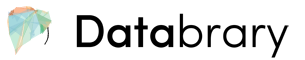
\includegraphics[height=4em]{img/databrary.png}}

%%%%%%%%%%%%%%%%%%%%%%%%%%%%%%%%%%%%%%%%%%%%%%%%%%%%%%%%%%%%%%%%%%%%%%%%%%%%%%
%%% Now define the boxes that make up the poster
%%%---------------------------------------------------------------------------
%%% Each box has a name and can be placed absolutely or relatively.
%%% The only inconvenience is that you can only specify a relative position 
%%% towards an already declared box. So if you have a box attached to the 
%%% bottom, one to the top and a third one which should be in between, you 
%%% have to specify the top and bottom boxes before you specify the middle 
%%% box.
%%%%%%%%%%%%%%%%%%%%%%%%%%%%%%%%%%%%%%%%%%%%%%%%%%%%%%%%%%%%

%%%%%%%%%%%%%%%%%%%%%%%%%%%%%%%%%%%%%%%%%%%%%%%%%%%%%%%%%%%%%%%%%%%%%%%%%%%%%%
  \headerbox{Motivation}{name=abstract,column=0,row=0}
%%%%%%%%%%%%%%%%%%%%%%%%%%%%%%%%%%%%%%%%%%%%%%%%%%%%%%%%%%%%%%%%%%%%%%%%%%%%%%  
    {
  Optic flow evokes different cortical activation patterns across the scalp depending on the pattern of flow (radial vs. linear) and speed. These effects are seen both in adults \cite{fesi_cortical_2014} and children \cite{gilmore_childrens_2016}. 
  This study examined whether the detection of optic flow in child observers varies by pattern and speed in similar ways to adults \cite{adamiak_adult_observer_2015}\cite{adamiak_adult_2015}, and the extent to which behavioral detection accords with patterns of brain activation.
    }

%%%%%%%%%%%%%%%%%%%%%%%%%%%%%%%%%%%%%%%%%%%%%%%%%%%%%%%%%%%%%%%%%%%%%%%%%%%%%%
  \headerbox{Acknowledgements}{name=thanks,column=0,below=abstract}
%%%%%%%%%%%%%%%%%%%%%%%%%%%%%%%%%%%%%%%%%%%%%%%%%%%%%%%%%%%%%%%%%%%%%%%%%%%%%%
    {
      This material is based upon work supported by the National Science Foundation under Grant Number BCS-1147440. Any opinions, findings, and conclusions or recommendations expressed in this material are those of the author(s) and do not necessarily reflect the views of the National Science Foundation. 
    }

%%%%%%%%%%%%%%%%%%%%%%%%%%%%%%%%%%%%%%%%%%%%%%%%%%%%%%%%%%%%%%%%%%%%%%%%%%%%%%
  \headerbox{Method}{name=method,column=0,below=thanks}
%%%%%%%%%%%%%%%%%%%%%%%%%%%%%%%%%%%%%%%%%%%%%%%%%%%%%%%%%%%%%%%%%%%%%%%%%%%%%%
    {
      Child observers (n=20; 5.3-8.5 years, 12 female) viewed two side-by-side, time varying (1.2 Hz coherent/incoherent cycle) annular-shaped (18 deg outer/5 deg inner diameter) optic flow displays at a viewing distance of 60 cm. One display depicted random (0\% coherent) motion while the other depicted radial or linear motion at one of four fixed coherence levels in one of two coherence level profiles (20, 40, 60, 80\%) or (15, 30, 45, 60\%). Observers fixated centrally and judged which side contained coherent motion, indicating the choice by pointing to the monitor. The choice was entered by the experimenter via keypress. Within a single run, speed was either 2 or 8 deg/s. Four runs were collected per participant in a single visit.
    }

% %%%%%%%%%%%%%%%%%%%%%%%%%%%%%%%%%%%%%%%%%%%%%%%%%%%%%%%%%%%%%%%%%%%%%%%%%%%%%%
   \headerbox{Data Sharing}{name=sharing,column=0, below=method, above=bottom}
% %%%%%%%%%%%%%%%%%%%%%%%%%%%%%%%%%%%%%%%%%%%%%%%%%%%%%%%%%%%%%%%%%%%%%%%%%%%%%%
     {
       Movies of the displays, metadata about the participants, and raw data files are available at \\
       \url{https://nyu.databrary.org/volume/218}.
     }

%%%%%%%%%%%%%%%%%%%%%%%%%%%%%%%%%%%%%%%%%%%%%%%%%%%%%%%%%%%%%%%%%%%%%%%%%%%%%%
  \headerbox{Displays}{name=displays,column=1,row=0}
%%%%%%%%%%%%%%%%%%%%%%%%%%%%%%%%%%%%%%%%%%%%%%%%%%%%%%%%%%%%%%%%%%%%%%%%%%%%%%
    {
      \vspace{3em}
      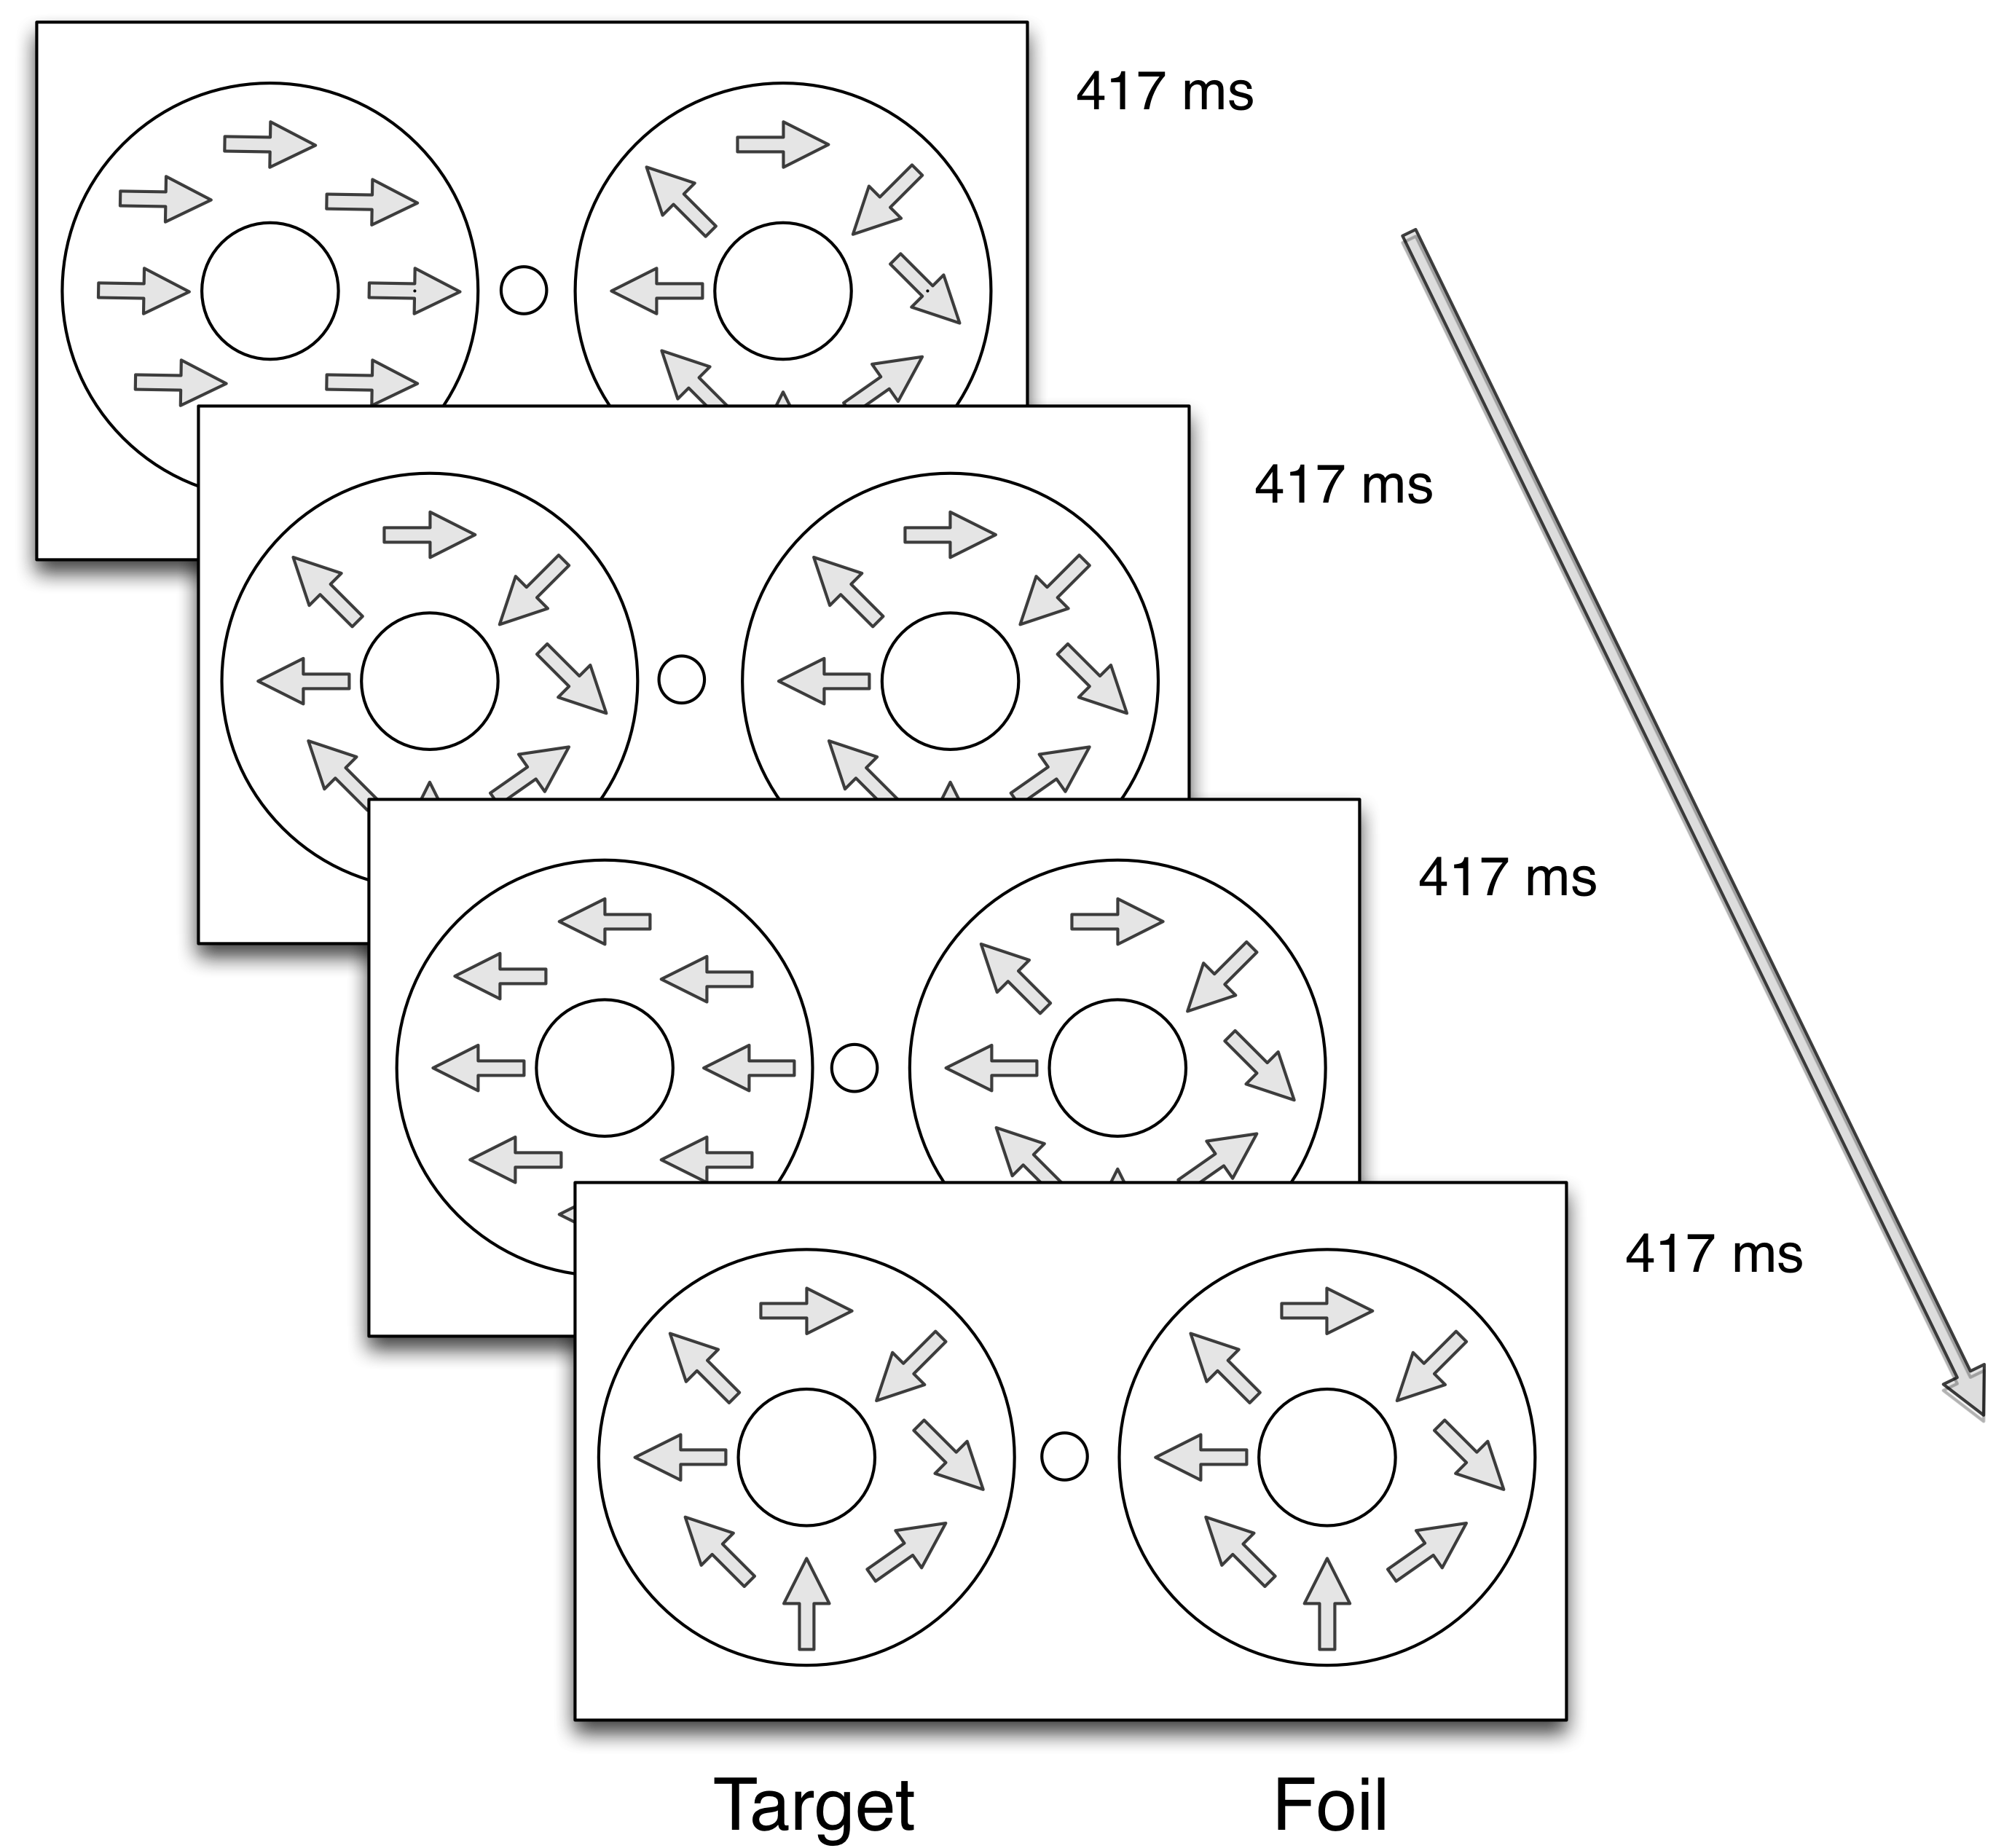
\includegraphics[scale=0.30]{img/optic-flow-psychophysics-display.png}
      \vspace{4em}
    }


%%%%%%%%%%%%%%%%%%%%%%%%%%%%%%%%%%%%%%%%%%%%%%%%%%%%%%%%%%%%%%%%%%%%%%%%%%%%%%
  \headerbox{References}{name=references,column=1, below=displays, above=bottom}
%%%%%%%%%%%%%%%%%%%%%%%%%%%%%%%%%%%%%%%%%%%%%%%%%%%%%%%%%%%%%%%%%%%%%%%%%%%%%%
    {
      \smaller
%For use with external .bib file
          \renewcommand{\refname}{\vspace{-0.5em}} % removes "References" canned text.
          \bibliographystyle{IEEEtran}
          \bibliography{IEEEabrv,poster_landscape}
     \vspace{0.3em}
    }

%%%%%%%%%%%%%%%%%%%%%%%%%%%%%%%%%%%%%%%%%%%%%%%%%%%%%%%%%%%%%%%%%%%%%%%%%%%%%%
  \headerbox{Results}{name=results,column=2,span=2,row=0, bottomaligned=references}
%%%%%%%%%%%%%%%%%%%%%%%%%%%%%%%%%%%%%%%%%%%%%%%%%%%%%%%%%%%%%%%%%%%%%%%%%%%%%%
    {
      We analyzed the proportion of correct responses and response times using generalized linear mixed effects modeling in R. As predicted, the proportion of correct judgments increased and the response times of correct judgements declined with increasing motion coherence. Fast optic flow patterns were perceived more reliably than slow, and radial patterns were perceived more reliably than linear patterns.
      
%      Coherence \(\chi^{2}(1)=1110.3, p<.0001\), pattern type \(\chi^{2}(1)=66.148, p<.0001\), cohererence by pattern type \(\chi^{2}(1)=69.879, p<.0001\), and speed \(\chi^{2}(1)=9.1834, p<.0024\) remained in the final model for proportion correct judgments. 
%      As coherence increased from 5 to 20\%, accuracy to detect radial flows increased from .55 to .98 and for translational flows from .59 to .89. 
%      We found comparable effects for reaction time.
      % There were main effects of coherence \emph{F}(1,471)=423.42, \emph{p}<.0001 and pattern \emph{F}(1,471)=9.94, \emph{p}<.002 on proportion correct judgments and a pattern by coherence interaction \emph{F}(1,471)=19.48, \emph{p}<.0001. 
      % For reaction time, there were main effects of coherence \emph{F}(1,455)=229.84, \emph{p}<.0001 and pattern \emph{F}(1,455)=10.55, \emph{p}<.0001, and a pattern by coherence interaction \emph{F}(1,455)=39.27, \emph{p}<.0001. 
%      Participants were \textbf{most accurate and fastest to detect slow radial flows}, and performance improved  rapidly as coherence increased.
      Combined with other prior EEG results, these data suggest that optic flow processing networks mature rapidly from infancy, but undergo less rapid, subtler change from mid-childhood to adulthood.

      \begin{center}
        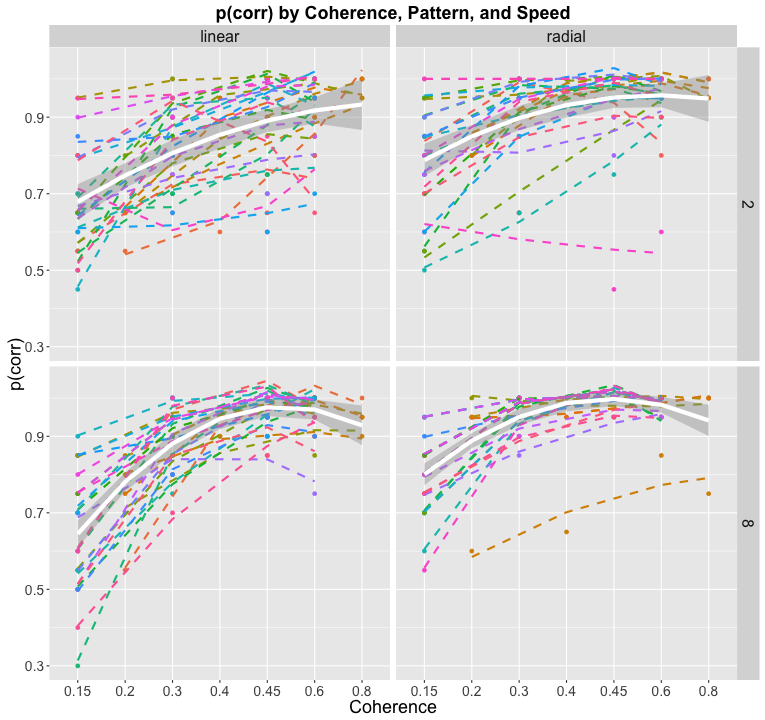
\includegraphics[scale=0.3]{img/plot-pcor-2.png}
     
        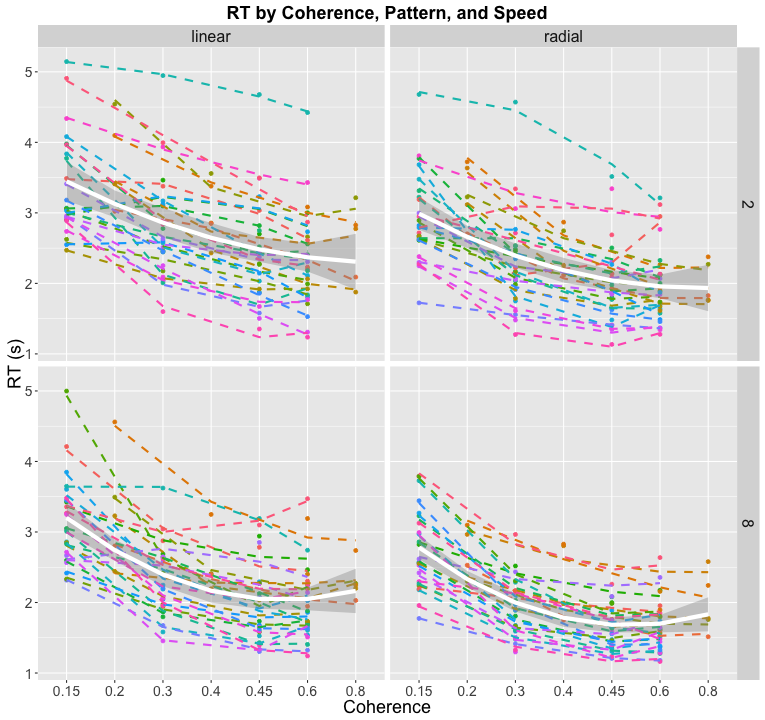
\includegraphics[scale=0.3]{img/plot-rt-2.png}
      \end{center}
    }


% %%%%%%%%%%%%%%%%%%%%%%%%%%%%%%%%%%%%%%%%%%%%%%%%%%%%%%%%%%%%%%%%%%%%%%%%%%%%%%
%   \headerbox{Future Directions}{name=future,column=1,aligned=references,above=bottom}
% %%%%%%%%%%%%%%%%%%%%%%%%%%%%%%%%%%%%%%%%%%%%%%%%%%%%%%%%%%%%%%%%%%%%%%%%%%%%%%
%     {
%       Taken together the results suggest that sensitivity to detect optic flow in noise varies by pattern type and speed in ways that partially map onto prior physiological results. 
%     }


\end{poster}

\end{document}
